\documentclass[russian,a4paper,12pt]{scrartcl}
\usepackage{babel}
\usepackage[utf8]{inputenc}
\usepackage[left=3cm,right=1cm,top=1cm,bottom=1cm]{geometry}
\usepackage{misccorr}
\usepackage{amsmath}
\usepackage{minted}
\usepackage{graphicx}
\usepackage{xcolor}
\usepackage{hyperref}
 % Цвета для гиперссылок
\definecolor{linkcolor}{HTML}{799B03} % цвет ссылок
\definecolor{urlcolor}{HTML}{799B03} % цвет гиперссылок
\hypersetup{pdfstartview=FitH,  linkcolor=blue,urlcolor=blue, colorlinks=true}

\begin{document}
	\begin{center}
	
		\large{МИНИСТЕРСТВО ОБРАЗОВАНИЯ И НАУКИ\\ РОССИЙСКОЙ ВЕДЕРАЦИИ} \par
		\bf\MakeUppercase{федеральное государственное автономное образовательное учреждение высшего образования} \par
		\textit{<<Санкт-Петербургский Государственный университет 
		Аэрокосмического Приборостроения>>} \par
	
	\vspace{10mm}
		
		\MakeUppercase{Кафедра №14} \par 
		
	\vspace{20mm}
	\begin{flushleft}
		{ОТЧЕТ}\par
		{ЗАЩИЩЕН С ОЦЕНКОЙ}\par
		{ПРЕПОДАВАТЕЛЬ}\par
	\end{flushleft}
	\begin{flushleft}
			\[
			\underset{\text{должность}}{\underline{\hspace{0.5cm}\text{\strut доц.,к.т.н.}\hspace{0.5cm}}}
			\quad\underset{\text{подпись, дата}}{\underline{\strut \hspace{4cm}}}
			\quad\underset{\text{инициалы, фамилия}}{\underline{\hspace{1cm}\text{\strut Н.В. Волошина}\hspace{1cm}}}
			\]
	\end{flushleft}
	\vspace{10mm}

		 \textbf{ОТЧЕТ О ЛАБОРАТОРНОЙ РАБОТЕ №3}\par{Графические фильтры}\par{По курсу: <<Основы мультимедия технологий>>.} \par
		
	\vspace{40mm}

	\begin{flushleft}
		{РАБОТУ ВЫПОЛНИЛ}\par
		\begin{flushleft}
			СТУДЕНТ ГРУППЫ 
			\underline{\strut 1441} 
			\quad\underset{\text{подпись, дата}}{\underline{\strut \hspace{3cm}}}\quad
			\underset{\text{инициалы, фамилия}}{\underline{\text{\strut А.А. Протасов}}}
		\end{flushleft}
	\end{flushleft}

	\vspace{50mm}
	
		{Санкт-Петербург\\ 2016}
	\thispagestyle{empty}
	\newpage
	
	\end{center}

	%\begin{flushleft}
	\section{Цель работы}
			Получение практических навыков реализации графических фильтров выполняющих преобразования изображений.
	\section{Постановка задачи}
			Для графических файлов в формате PNG реализовать фильтры выполняющие заданные преобразования изображения. Построить гистограммы для исходного и преобразованного изображений.\\
			Графические файлы для проверки изображений создать самостоятельно.
	\section{Задание}
			Черно-белый, Фильтр яркость/контраст, Медианный фильтр
	\section{Краткие теоритические сведения}
			PNG - растровый формат хранения графической информации, использующий сжатие без потерь по алгоритму Deflate.\\
			Deflate — это алгоритм сжатия без потерь, использующий комбинацию алгоритмов LZ77 и Хаффмана. Изначально был описан Филом Кацем для второй версии его архиватора PKZIP, который впоследствии был определён в RFC 1951[1] (1996 год).\\
			Гистогра́мма изображе́ния (иногда: график уровней или просто уровни) — гистограмма уровней насыщенности изображения (суммарная, или разделённая по цветовым каналам).\\

			Гистограмма изображения позволяет оценить количество и разнообразие оттенков изображения, а также общий уровень яркости изображения.\\
			Яркость — световая характеристика тел. Отношение силы света, излучаемого поверхностью, к площади ее проекции на плоскости, перпендикулярной оси наблюдения.\\
			Контрастность — различимость предмета наблюдения от окружающего его фона (монохроматическое излучение); цветовая контрастность — разновидность оптической контрастности, связанная с разницей цветовых оттенков.\\
			
			Иначе яроксть и контрастность можно описать так:\\
			Яркость — количество белого цвета на вашем фото. Чем выше вы ставите яркость, тем светлее становится изображение, соответственно в обратную сторону оно будет темнее до черного.\\
			Контрастность - разница между оттенками цвета предмета наблюдения и окружающего его фона. Если сформулировать проще то, это разница между различными расположенными рядом цветами. Чем выше контрастность, тем более резко мы наблюдаем переход от одного цвета к другому.\\
			
			Контрастность была реализована по следующим формулам[2]:\\
			\begin{center}
				$C=(\frac{100.0 + T}{100.0})^2$(1)
			\end{center}
			где С - коэффициент контрастности, а T- это значение от -100 до 100.
			\begin{center}
				$RGB = (((\frac{RGB^1}{255}-0.5)\cdot C)+0.5)\cdot 255$(2)
			\end{center}
			где RGB - компоненты красного, зеленого, синего пикселя, а C - это коэффициент из формулы (1)
		
			Черно-белый фильтр - преобразование изображения в черно-белую гамму(каждый цветовой канал пикселя имеет одно значение).\\
			Вычисляется по формуле[3] $\gamma = 0.299R + 0.587G + 0.144B$, где $\gamma$ - новое значение компоненты, $R, G, B$ - компоненты красного, зеленого и синего палитр.\\

			Медианный фильтр - один из видов цифровых фильтров, широко используемый в цифровой обработке сигналов и изображений для уменьшения уровня шума. Медианный фильтр является нелинейным КИХ-фильтром.\\
			Для упрощения дальнейшего рассмотрения ограничимся примером фильтра с квадратной маской размером $N*N$, при $N=3$. Скользящий фильтр просматривает отсчеты изображения слева-направо и сверху-вниз, при этом входную двумерную последовательность также представим в виде последовательного числового ряда отсчетов ${x(n)}$ слева-направо сверху-вниз. Из этой последовательности в каждой текущей точке маска фильтра выделяет массив $w(n)$, как $w$-элементный вектор, который в данном случае содержит все элементы из окна $3*3$, центрированные вокруг $x(n)$, и сам центральный элемент, если это предусмотрено типом маски:
			\begin{center}
			$w(n)=[x_1(n),x_2(n),...,x_W(n)]$(3)
			\end{center}
			В этом случае значения $x_i$
			соответствует отображению слева-направо и сверху-вниз окна $3*3$
			в одномерный вектор, как показано на рис. 1.\\
			\begin{center}
			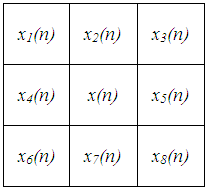
\includegraphics[scale=0.8]{matrix}\\ Рис. 1
			\end{center}
			Элементы данного вектора должны быть упорядочены в ряд по возрастанию или убыванию своих значений:
			\begin{center}
			$r(n)=[r_1(n),r_2(n),...,r_W(n)]$(4)
			\end{center}
			Определено значение медианы $y(n)=med(r(n))$, центральный отсчет маски заменен значением медианы. Если по типу маски центральный отсчет не входит в число ряда (3), то медианное значение находится в виде среднего значения двух центральных отсчетов ряда (4).
			Приведенные выражения не объясняют способа нахождения выходного сигнала вблизи конечных и пограничных точек в конечных последовательностях и изображениях. Один из простых приемов состоит в том, что нужно находить медиану только тех точек внутри изображения, которые попадают в пределы апертуры. Поэтому для точек, расположенных рядом с границами, медианы будут определены, исходя из меньшего числа точек. 
	\section{Описание метода реализации}
			Программа была написана в среде для разработки Qt[4] с использованием языка C++[5], фреймворка Qt[6] версии 5.7 и использованием библиотеки компьютерного зрения \\ OpenCV[7] версии 2.4.13.1.\\
			Для работы с изображениями были использованы следующие виды избражений: \\ 32-бита(класс QImage - Qt) и 8-бит(класс Mat - OpenCV).\\
			Для открытия изображения была использована стандартная функция imread() из библиотеки OpenCV. Так же для хранения изображения помимо типа Mat - библиотека OpenCV, был испльзован тип QImage - библиотека Qt, для взаимодействия между двумя разными способами храниния избражений, были написаны две функции конвертирования QImageToMat - из представления Qt в OpenCV и MatToQImage - соответственно наоборот. Для разделения изображения на разные цветовые палитры был использован vector[8] - контейнер из STL и стандартная функция split из библиотеки OpenCV.
	\newpage
	\section{Листинги}
	\usemintedstyle{autumn}
	\subsection{\text{Тело основной функции}}
		\inputminted[
			frame=lines,
			framesep=2mm,
			baselinestretch=1.2,
			fontsize=\footnotesize,
			linenos
			]{cpp}{main.cpp}
	\subsection{\text{Заголовок класса главного окна}}
		\inputminted[
			frame=lines,
			framesep=2mm,
			baselinestretch=1.2,
			fontsize=\footnotesize,
			linenos
			]{cpp}{mainwindow.h}
	\subsection{\text{Описание методов класса главного окна}}
		\inputminted[
			frame=lines,
			framesep=2mm,
			baselinestretch=1.2,
			fontsize=\footnotesize,
			linenos
			]{cpp}{mainwindow.cpp}
	\subsection{\text{Заголовок окна гистограммы}}
		\inputminted[
			frame=lines,
			framesep=2mm,
			baselinestretch=1.2,
			fontsize=\footnotesize,
			linenos
			]{cpp}{histogram.h}
	\subsection{\text{Описание методов класса окна гистограммы}}
		\inputminted[
			frame=lines,
			framesep=2mm,
			baselinestretch=1.2,
			fontsize=\footnotesize,
			linenos
			]{cpp}{histogram.cpp}
	\section{Примеры работы программы}
	\begin{center}
		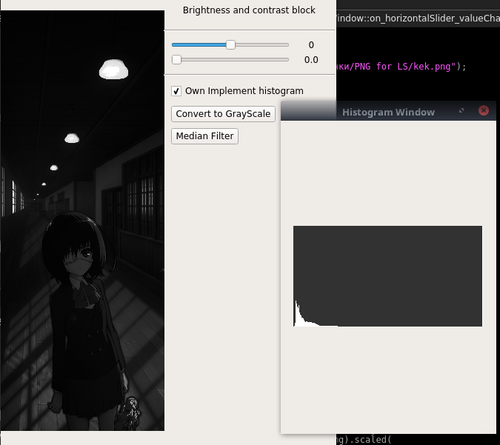
\includegraphics{kek}\\ \text{Черно-белый}\\
		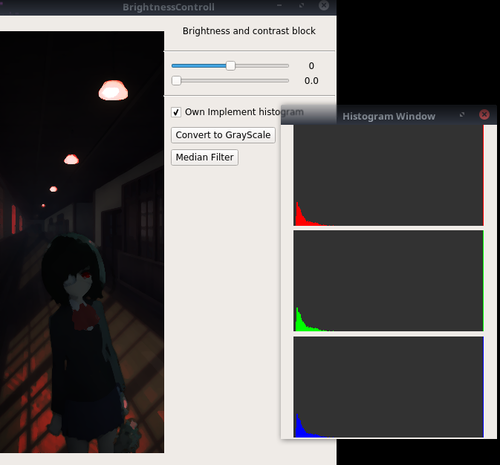
\includegraphics{kek1}\\ \text{Медианный}\\
		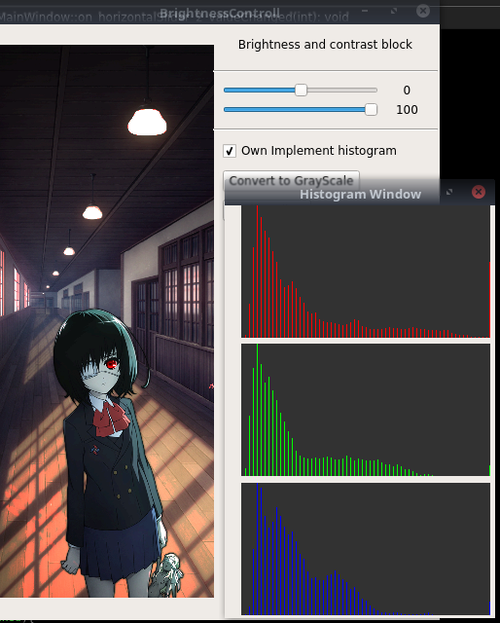
\includegraphics{kek2}\\ \text{Контрастность}
	\end{center}
	\newpage
	\begin{thebibliography}{15}
		\bibitem{Deflate}\href{https://tools.ietf.org/html/rfc1951#ref-1}{\underline{https://tools.ietf.org/html/rfc1951#ref-1}}
		\bibitem{Contrast-Brightness}\href{https://softwarebydefault.com/2013/04/20/image-contrast/}{\underline{https://softwarebydefault.com/2013/04/20/image-contrast/}}
		\bibitem{GRAYSCALE}\href{https://ru.wikipedia.org/wiki/Оттенки\_серого}{\underline{https://ru.wikipedia.org/wiki/Оттенки\_серого}}
		\bibitem{Shlee-2015}Шлее М. Qt 5.3. Профессиональное программирование на C++ \newblock --- Санкт-Петербург:
		Изд.  БХВ-Петербург, 2015. 928~с.
		\bibitem{C++-reference} \href{http://en.cppreference.com/w/}{\underline{http://en.cppreference.com/w/}}
		\bibitem{Qt-reference} \href{http://doc.qt.io/qt-5/reference-overview.html}{\underline{http://doc.qt.io/qt-5/reference-overview.html}}
		\bibitem{OpenCV-reference} \href{http://opencv.org/}{\underline{http://opencv.org/}}
		\bibitem{Vector} \href{http://en.cppreference.com/w/cpp/container/vector}{\underline{http://en.cppreference.com/w/cpp/container/vector}}
	\end{thebibliography}
\end{document}